\documentclass[aspectratio=169]{beamer}
% Add slides directory to search path for Dartmouth theme
\makeatletter
\def\input@path{{../}}
\makeatother
\usetheme{Dartmouth}

% Packages
\usepackage{fontspec}
\usepackage{listings}
\usepackage{xcolor}
\usepackage{tcolorbox}
\usepackage{booktabs}
\usepackage{hyperref}
\usepackage{tikz}
\usetikzlibrary{shapes,arrows,positioning,calc,automata}

% Font settings
\setmonofont{Courier New}

% Code listing settings
\lstset{
    language=Python,
    basicstyle=\ttfamily\small,
    keywordstyle=\color{blue},
    commentstyle=\color{gray},
    stringstyle=\color{red},
    showstringspaces=false,
    breaklines=true,
    frame=single,
    numbers=left,
    numberstyle=\tiny\color{gray}
}

% Custom colors
\definecolor{thinkbox}{RGB}{255,245,220}
\definecolor{discussbox}{RGB}{230,240,255}

% Custom boxes
\newtcolorbox{thinkaboutit}{
    colback=thinkbox,
    colframe=orange,
    title=💭 Think about it!,
    fonttitle=\bfseries
}

\newtcolorbox{discussion}{
    colback=discussbox,
    colframe=blue,
    title=💬 Discussion,
    fonttitle=\bfseries
}

% Title page information
\title{Lecture 2: Pattern Matching \& ELIZA}
\subtitle{The Fundamentals of Conversational AI 🔧}
\author{PSYC 51.07: Models of Language and Communication}
\institute{Dr. Jeremy R. Manning}
\date{Week 1 - Day 2}

\begin{document}

% Title slide
\begin{frame}[shrink=10]
\titlepage
\end{frame}

% Table of contents
\begin{frame}[shrink=5]{Today's Journey 🗺️}
\tableofcontents
\end{frame}

\section{Recap: Language vs. Understanding}

\begin{frame}{Last Time... 🔄}
\small
\begin{block}{Key Ideas from Lecture 1}
\begin{itemize}\setlength{\itemsep}{0pt}
    \item Consciousness is complex and hard to define
    \item Language and thought are separable but interactive
    \item Current LLMs are not conscious
    \item Pattern matching can create illusions of understanding
\end{itemize}
\end{block}

\vspace{0.3cm}

\begin{discussion}
Today we'll see \textit{how} pattern matching can create these illusions by building our own simple conversational system!
\end{discussion}
\end{frame}

\section{How Computers Process Language}

\begin{frame}[shrink=5]{The Fundamental Challenge 💻}
\begin{block}{Core Problem}
Computers don't "understand" meaning—they manipulate \textbf{strings of characters}.
\end{block}

\vspace{0.3cm}

\begin{center}
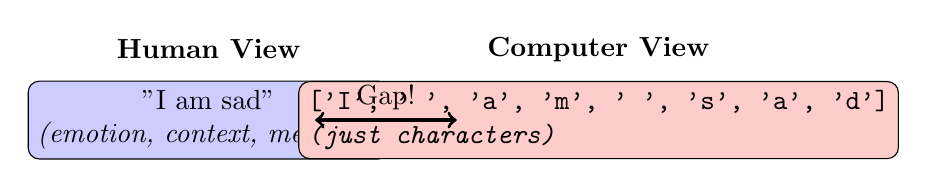
\begin{tikzpicture}[scale=0.9]
% Human view
\node at (0,3) {\textbf{Human View}};
\node[draw, rounded corners, fill=blue!20, align=center] at (0,2) {
    "I am sad"\\
    \textit{(emotion, context, meaning)}
};

% Computer view
\node at (5.5,3) {\textbf{Computer View}};
\node[draw, rounded corners, fill=red!20, font=\ttfamily, align=left] at (5.5,2) {
    ['I', ' ', 'a', 'm', ' ', 's', 'a', 'd']\\
    \textit{(just characters)}
};

% Arrow between
\draw[<->, very thick] (1.5,2) -- (3.5,2);
\node[above] at (2.5,2) {Gap!};
\end{tikzpicture}
\end{center}

\vspace{0.3cm}

\textbf{The question:} How do we bridge this gap?
\end{frame}

\begin{frame}{Everything Starts with Patterns 🎯}
\small
\textbf{Basic text operations:}
\begin{enumerate}\setlength{\itemsep}{0pt}
    \item \textbf{Finding} specific words or phrases
    \item \textbf{Replacing} parts of text
    \item \textbf{Extracting} information
    \item \textbf{Transforming} input to output
\end{enumerate}

\vspace{0.3cm}

\begin{alertblock}{Important Insight}
Even sophisticated models like GPT-4 are (at their core) doing \textit{pattern matching}—just at a much more complex level!
\end{alertblock}

\vspace{0.3cm}

\begin{thinkaboutit}
If you can master simple patterns, you'll understand the foundations of ALL natural language processing!
\end{thinkaboutit}
\end{frame}

\section{String Manipulation Basics}

\begin{frame}[fragile]{Simple String Replacement 🔧}
\textbf{Example 1: Direct replacement}

\begin{lstlisting}
user_input = "I am feeling sad"
response = user_input.replace("I am", "Why are you")
print(response)
# Output: "Why are you feeling sad"
\end{lstlisting}

\vspace{0.3cm}

\textbf{What happened here?}
\begin{itemize}\setlength{\itemsep}{0pt}
    \item Found the substring "I am"
    \item Replaced it with "Why are you"
    \item Everything else stayed the same
\end{itemize}

\vspace{0.3cm}

\begin{thinkaboutit}
This seems intelligent! But is it? What are the limitations?
\end{thinkaboutit}
\end{frame}

\begin{frame}[fragile]{The Problem with Direct Replacement ❌}
\textbf{What if the input is slightly different?}

\begin{lstlisting}
# Works
user_input = "I am sad"
response = user_input.replace("I am", "Why are you")
# "Why are you sad" ✓

# Doesn't work
user_input = "I'm sad"
response = user_input.replace("I am", "Why are you")
# "I'm sad" (unchanged!) ✗

# Doesn't work
user_input = "I am very very sad"
response = user_input.replace("I am", "Why are you")
# "Why are you very very sad"
# (But we only wanted to capture "sad") ✗
\end{lstlisting}

\vspace{0.3cm}

\textbf{Solution:} We need more flexible patterns! → \textbf{Regular Expressions}
\end{frame}

\section{Regular Expressions (Regex)}

\begin{frame}[fragile]{Introduction to Regular Expressions 🎯}
\begin{block}{What are Regular Expressions?}
A powerful language for describing patterns in text, not just exact matches.
\end{block}

\vspace{0.3cm}

\textbf{Example: Matching with wildcards}

\begin{lstlisting}
import re

pattern = r"I am (.*)"
match = re.search(pattern, "I am feeling sad")

if match:
    feeling = match.group(1)  # Captures "feeling sad"
    response = f"Why are you {feeling}?"
    print(response)
# Output: "Why are you feeling sad?"
\end{lstlisting}

\vspace{0.3cm}

\textbf{Key: } The \texttt{(.*)} captures \textit{anything} after "I am"!
\end{frame}

\begin{frame}{Regex Syntax Basics 📝}
\begin{center}
\begin{tabular}{lll}
\toprule
\textbf{Pattern} & \textbf{Meaning} & \textbf{Example} \\
\midrule
\texttt{.} & Any single character & \texttt{c.t} matches "cat", "cut" \\
\texttt{*} & Zero or more of previous & \texttt{ca*t} matches "ct", "cat", "caat" \\
\texttt{+} & One or more of previous & \texttt{ca+t} matches "cat", "caat" \\
\texttt{?} & Zero or one of previous & \texttt{ca?t} matches "ct", "cat" \\
\texttt{()} & Capture group & \texttt{(cat)} captures "cat" \\
\texttt{|} & Or & \texttt{cat|dog} matches "cat" or "dog" \\
\texttt{[]} & Character class & \texttt{[abc]} matches "a", "b", or "c" \\
\texttt{\^{}} & Start of string & \texttt{\^{}cat} matches "cat" at start \\
\texttt{\$} & End of string & \texttt{cat\$} matches "cat" at end \\
\bottomrule
\end{tabular}
\end{center}

\vspace{0.3cm}

\begin{alertblock}{Practice Makes Perfect}
Regex can be tricky at first, but it's an essential skill for NLP!
\end{alertblock}
\end{frame}

\begin{frame}[fragile]{Regex Examples 💡}
\begin{columns}
\begin{column}{0.5\textwidth}
\textbf{Example 1: Email addresses}
\begin{lstlisting}[basicstyle=\ttfamily\tiny]
pattern = r"\w+@\w+\.\w+"
text = "Email: joe@example.com"
match = re.search(pattern, text)
# Matches: joe@example.com
\end{lstlisting}

\vspace{0.15cm}

\textbf{Example 2: Phone numbers}
\begin{lstlisting}[basicstyle=\ttfamily\tiny]
pattern = r"\d{3}-\d{3}-\d{4}"
text = "Call 555-123-4567"
match = re.search(pattern, text)
# Matches: 555-123-4567
\end{lstlisting}
\end{column}

\begin{column}{0.5\textwidth}
\textbf{Example 3: Multiple captures}
\begin{lstlisting}[basicstyle=\ttfamily\tiny]
pattern = r"I (.*) my (.*)"
text = "I love my family"
match = re.search(pattern, text)
if match:
    verb = match.group(1)   # "love"
    obj = match.group(2)    # "family"
\end{lstlisting}

\vspace{0.15cm}

\textbf{Example 4: Optional parts}
\begin{lstlisting}[basicstyle=\ttfamily\tiny]
pattern = r"I'?m? (sad|happy)"
# Matches: "I am sad", "I'm sad",
#          "I am happy", "I'm happy"
\end{lstlisting}
\end{column}
\end{columns}

\vspace{0.3cm}

\begin{thinkaboutit}
With these patterns, we can handle much more variation in user input!
\end{thinkaboutit}
\end{frame}

\begin{frame}[fragile]{Capturing and Using Patterns 🎯}
\textbf{The power of capture groups:}

\begin{lstlisting}
pattern = r"I (.*) my (.*)"
match = re.search(pattern, "I love my family")

if match:
    verb = match.group(1)      # "love"
    object = match.group(2)    # "family"
    response = f"Tell me more about your {object}."
    print(response)
# Output: "Tell me more about your family."
\end{lstlisting}

\vspace{0.3cm}

\begin{thinkaboutit}
This is remarkably simple, yet it can create the \textit{illusion} of understanding! The bot seems to know what you're talking about!
\end{thinkaboutit}
\end{frame}

\begin{frame}[shrink=5]{Regex State Machine Visualization 🔧}
\begin{center}
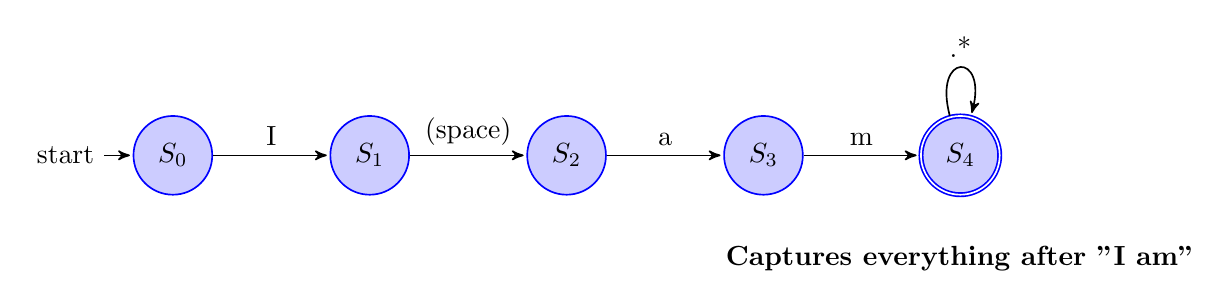
\begin{tikzpicture}[scale=0.8, ->, >=stealth', shorten >=1pt, auto, node distance=2.5cm, semithick]
\tikzstyle{every state}=[fill=blue!20, draw=blue, text=black, minimum size=1cm]

% Pattern: I am (.*)
\node[state, initial] (s0) {$S_0$};
\node[state] (s1) [right of=s0] {$S_1$};
\node[state] (s2) [right of=s1] {$S_2$};
\node[state] (s3) [right of=s2] {$S_3$};
\node[state, accepting] (s4) [right of=s3] {$S_4$};

\path (s0) edge node {I} (s1)
      (s1) edge node {(space)} (s2)
      (s2) edge node {a} (s3)
      (s3) edge node {m} (s4)
      (s4) edge [loop above] node {.*} (s4);

\node[below=0.5cm of s4] {\textbf{Captures everything after "I am"}};
\end{tikzpicture}
\end{center}

\vspace{0.3cm}

\begin{block}{How It Works}
The regex engine steps through the input character by character, tracking which state it's in. When it matches the pattern, it captures the specified groups.
\end{block}
\end{frame}

\section{Pre and Post Substitutions}

\begin{frame}[fragile]{Pre-Substitutions: Normalizing Input 🔄}
\begin{block}{Why Pre-Substitutions?}
Users type in many different ways. We need to normalize input before pattern matching.
\end{block}

\vspace{0.3cm}

\begin{lstlisting}
pre_subs = {
    "dont": "don't",
    "cant": "can't",
    "wont": "won't",
    "im": "I'm",
    "youre": "you're"
}

user_input = "I dont know"
for old, new in pre_subs.items():
    user_input = user_input.replace(old, new)
# Result: "I don't know"
\end{lstlisting}

\vspace{0.3cm}

\textbf{Benefit:} Now our patterns can assume standardized input!
\end{frame}

\begin{frame}[fragile]{Post-Substitutions: Fixing Grammar 🔄}
\begin{block}{Why Post-Substitutions?}
When we mirror user input, we need to flip pronouns and verb forms.
\end{block}

\vspace{0.3cm}

\begin{lstlisting}
post_subs = {
    " i ": " you ",
    " my ": " your ",
    " am ": " are ",
    " was ": " were ",
    " I ": " you "
}

# User said: "I am sad"
# We extracted: "am sad"
# Initial response: "Why are you am sad" (WRONG!)

response = " Why are you am sad "
for old, new in post_subs.items():
    response = response.replace(old, new)
# Result: "Why are you are sad" (BETTER!)
\end{lstlisting}

\vspace{0.3cm}

\textbf{Note:} This is still imperfect, but good enough for ELIZA!
\end{frame}

\begin{frame}[shrink=5]{The Substitution Pipeline 🔧}
\begin{center}
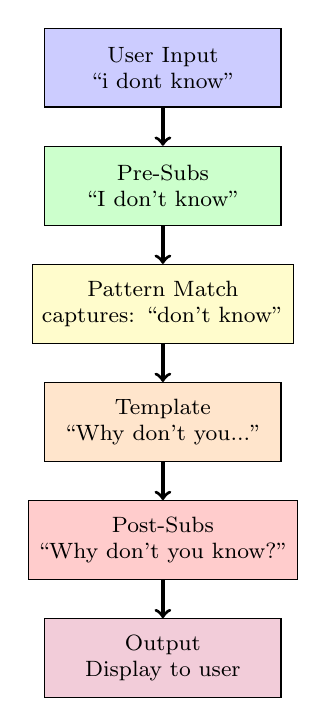
\begin{tikzpicture}[scale=0.85,
    node distance=1.5cm,
    every node/.style={font=\footnotesize},
    box/.style={rectangle, draw, fill=blue!20, minimum width=3cm, minimum height=1cm, align=center}
]

% Pipeline
\node[box] (input) {User Input\\``i dont know''};
\node[box, below of=input, fill=green!20] (pre) {Pre-Subs\\``I don't know''};
\node[box, below of=pre, fill=yellow!20] (pattern) {Pattern Match\\captures: ``don't know''};
\node[box, below of=pattern, fill=orange!20] (template) {Template\\``Why don't you...''};
\node[box, below of=template, fill=red!20] (post) {Post-Subs\\``Why don't you know?''};
\node[box, below of=post, fill=purple!20] (output) {Output\\Display to user};

% Arrows
\draw[->, very thick] (input) -- (pre);
\draw[->, very thick] (pre) -- (pattern);
\draw[->, very thick] (pattern) -- (template);
\draw[->, very thick] (template) -- (post);
\draw[->, very thick] (post) -- (output);

\end{tikzpicture}
\end{center}
\end{frame}

\section{Introduction to ELIZA}

\begin{frame}{ELIZA: A Revolutionary Program 🎭}
\small
\begin{columns}
\begin{column}{0.6\textwidth}
\begin{block}{Weizenbaum (1966)}
\textit{ELIZA — A Computer Program For the Study of Natural Language Communication Between Man and Machine}
\end{block}

\vspace{0.15cm}

\textbf{What was ELIZA?}
\begin{itemize}\setlength{\itemsep}{0pt}
    \item First "chatbot" (1964-1966)
    \item Simulated a Rogerian psychotherapist
    \item Used pattern matching \& string manipulation
    \item Created by Joseph Weizenbaum at MIT
\end{itemize}
\end{column}

\begin{column}{0.4\textwidth}
\begin{thinkaboutit}
ELIZA was meant to \textit{demonstrate} the superficiality of human-computer interaction.

Instead, people became emotionally attached to it!
\end{thinkaboutit}
\end{column}
\end{columns}
\end{frame}

\begin{frame}{Why a Rogerian Therapist? 🧠}
\small
\begin{block}{Carl Rogers' Approach}
Rogerian therapy is \textit{non-directive}—the therapist mainly reflects what the patient says back to them.
\end{block}

\vspace{0.3cm}

\textbf{Perfect for a chatbot because:}
\begin{itemize}\setlength{\itemsep}{0pt}
    \item ✅ Doesn't require understanding the problem
    \item ✅ Can use simple reflection ("Tell me more about X")
    \item ✅ Asks open-ended questions
    \item ✅ Minimal need for world knowledge
    \item ✅ Pattern matching is sufficient!
\end{itemize}

\vspace{0.3cm}

\begin{discussion}
\textbf{Patient:} I'm sad about my mother.\\
\textbf{Therapist:} Tell me more about your mother.\\
\textbf{Pattern:} \texttt{I am (.*) about my (.*)}\\
\textbf{Response:} \texttt{Tell me more about your \{2\}.}
\end{discussion}
\end{frame}

\begin{frame}[shrink=5]{How ELIZA Works: High Level 🔧}
\begin{center}
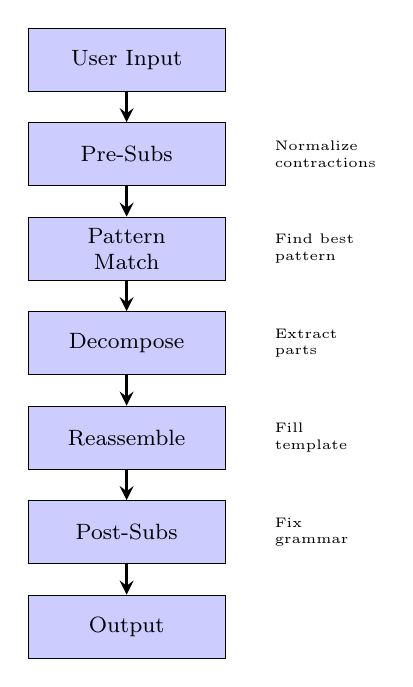
\begin{tikzpicture}[scale=0.85,
    node distance=1.2cm,
    box/.style={rectangle, draw, fill=blue!20, minimum width=2.5cm, minimum height=0.8cm, align=center, font=\footnotesize},
    arrow/.style={->, >=stealth, very thick}
]

% Main flow
\node[box] (input) {User Input};
\node[box, below of=input] (pre) {Pre-Subs};
\node[box, below of=pre] (match) {Pattern\\Match};
\node[box, below of=match] (decompose) {Decompose};
\node[box, below of=decompose] (reassemble) {Reassemble};
\node[box, below of=reassemble] (post) {Post-Subs};
\node[box, below of=post] (output) {Output};

% Arrows
\draw[arrow] (input) -- (pre);
\draw[arrow] (pre) -- (match);
\draw[arrow] (match) -- (decompose);
\draw[arrow] (decompose) -- (reassemble);
\draw[arrow] (reassemble) -- (post);
\draw[arrow] (post) -- (output);

% Side annotations
\node[right=0.5cm of pre, font=\tiny, align=left] {Normalize\\contractions};
\node[right=0.5cm of match, font=\tiny, align=left] {Find best\\pattern};
\node[right=0.5cm of decompose, font=\tiny, align=left] {Extract\\parts};
\node[right=0.5cm of reassemble, font=\tiny, align=left] {Fill\\template};
\node[right=0.5cm of post, font=\tiny, align=left] {Fix\\grammar};

\end{tikzpicture}
\end{center}

\begin{alertblock}{No Understanding Required!}
ELIZA had \textbf{zero} understanding. It's pure pattern transformation!
\end{alertblock}
\end{frame}

\begin{frame}[shrink=10]{Pattern Priority and Ranking 🎯}
\small
\begin{block}{Multiple Pattern Problem}
What if more than one pattern matches the input?
\end{block}

\vspace{0.3cm}

\textbf{Example input:} "I am sad about my mother"

\textbf{Multiple matches:}
\begin{itemize}\setlength{\itemsep}{0pt}
    \item Pattern 1: \texttt{I am (.*)} - Very general
    \item Pattern 2: \texttt{(.*) mother (.*)} - Specific keyword
    \item Pattern 3: \texttt{I am (.*) about (.*)} - More specific
\end{itemize}

\vspace{0.3cm}

\textbf{ELIZA's solution:}
\begin{enumerate}\setlength{\itemsep}{0pt}
    \item Each pattern has a \textbf{rank} (priority score)
    \item Keywords like "mother", "father", "family" get higher ranks
    \item More specific patterns generally rank higher
    \item Choose the highest-ranking pattern that matches
\end{enumerate}
\end{frame}

\begin{frame}[fragile]{ELIZA Pattern Structure 📋}
\textbf{A typical ELIZA rule:}

\begin{lstlisting}[language=Python, basicstyle=\ttfamily\tiny]
{
    "pattern": r"(.*) my (mother|father|family) (.*)",
    "rank": 100,  # High priority for family keywords
    "responses": [
        "Tell me more about your {2}.",
        "How do you feel about your {2}?",
        "What role does your {2} play in this?",
        "Does your {2} influence how you feel?"
    ]
}
\end{lstlisting}

\vspace{0.3cm}

\textbf{How it works:}
\begin{enumerate}\setlength{\itemsep}{0pt}
    \item \texttt{pattern}: Regex to match input
    \item \texttt{rank}: Priority level (higher = more important)
    \item \texttt{responses}: List of possible response templates
    \item \texttt{\{2\}}: Placeholder for captured group 2
\end{enumerate}
\end{frame}

\begin{frame}{Example ELIZA Conversation 💬}
\begin{block}{Sample Interaction}
\textbf{ELIZA:} Welcome. What brings you here today?

\textbf{User:} I am feeling sad.

\textbf{ELIZA:} Why do you feel sad?

\textbf{User:} I can't stop thinking about my family.

\textbf{ELIZA:} Tell me more about your family.

\textbf{User:} My mother never understood me.

\textbf{ELIZA:} Who else in your family never understood you?

\textbf{User:} I have to go now.

\textbf{ELIZA:} That will be \$200. See you again next week.
\end{block}
\end{frame}

\begin{frame}[shrink=10]{Breaking Down the Conversation 🔍}
\textbf{Let's analyze what happened:}

\vspace{0.3cm}

\begin{enumerate}\setlength{\itemsep}{0pt}
    \item \textbf{User:} "I am feeling sad"
    \begin{itemize}\setlength{\itemsep}{0pt}
        \item Pattern: \texttt{I am (.*)}
        \item Captures: "feeling sad"
        \item Response template: "Why do you \{1\}?"
    \end{itemize}

    \vspace{0.2cm}

    \item \textbf{User:} "I can't stop thinking about my family"
    \begin{itemize}\setlength{\itemsep}{0pt}
        \item Pattern: \texttt{(.*) my family (.*)}
        \item Higher rank due to keyword "family"
        \item Response: "Tell me more about your family."
    \end{itemize}

    \vspace{0.2cm}

    \item \textbf{User:} "My mother never understood me"
    \begin{itemize}\setlength{\itemsep}{0pt}
        \item Pattern: \texttt{my (mother|father) (.*) me}
        \item Response: "Who else in your family \{2\} you?"
        \item Post-sub: "me" stays "you"
    \end{itemize}
\end{enumerate}
\end{frame}

\section{The Power of Simple Patterns}

\begin{frame}{Why Does This Work? 🤔}
\small
\begin{block}{The Psychology Behind ELIZA}
Humans are pattern-seeking creatures who project understanding onto machines.
\end{block}

\vspace{0.3cm}

\textbf{Factors that create the illusion:}
\begin{enumerate}\setlength{\itemsep}{0pt}
    \item \textbf{Context}: We assume the bot understands context
    \item \textbf{Expectations}: We expect intelligence from human-like responses
    \item \textbf{Language structure}: Natural language has inherent patterns
    \item \textbf{Confirmation bias}: We remember hits, forget misses
    \item \textbf{Anthropomorphization}: We attribute human qualities to machines
\end{enumerate}

\vspace{0.3cm}

\begin{thinkaboutit}
The "intelligence" is often in the \textit{interpreter} (you!), not the program!
\end{thinkaboutit}
\end{frame}

\begin{frame}{When Pattern Matching Fails 💥}
\begin{block}{Example Failure Cases}
\textbf{User:} My mother and father are fighting.\\
\textbf{ELIZA:} Tell me more about your father. \textit{(Only caught "father")}

\vspace{0.2cm}

\textbf{User:} I saw a mother duck with her babies.\\
\textbf{ELIZA:} Tell me more about your mother. \textit{(Wrong context!)}

\vspace{0.2cm}

\textbf{User:} Why do you keep asking about my family?\\
\textbf{ELIZA:} Tell me more about your family. \textit{(Recursive failure)}
\end{block}

\vspace{0.3cm}

\begin{alertblock}{Important Lesson}
Pattern matching works surprisingly well, but it fundamentally lacks understanding. It can't handle context, sarcasm, or complex reasoning.
\end{alertblock}
\end{frame}

\begin{frame}[shrink=5]{Comparison: ELIZA vs Modern LLMs 📊}
\begin{center}
\begin{tikzpicture}[scale=0.85]
% Create comparison table
\node at (0,4) {\textbf{Capability}};
\node at (3,4) {\textbf{ELIZA (1966)}};
\node at (7,4) {\textbf{GPT-4 (2023)}};

\draw[thick] (-1.5,3.7) -- (8.5,3.7);

% Rows
\node[left] at (-1,3) {Pattern matching};
\node at (3,3) {✓ Simple regex};
\node at (7,3) {✓ Neural patterns};

\node[left] at (-1,2.2) {Learning};
\node at (3,2.2) {✗ Hand-coded};
\node at (7,2.2) {✓ From data};

\node[left] at (-1,1.4) {Context};
\node at (3,1.4) {✗ None};
\node at (7,1.4) {✓ Long-range};

\node[left] at (-1,0.6) {World knowledge};
\node at (3,0.6) {✗ None};
\node at (7,0.6) {✓ Extensive};

\node[left] at (-1,-0.2) {Semantic understanding};
\node at (3,-0.2) {✗ None};
\node at (7,-0.2) {❓ Debated};

\node[left] at (-1,-1) {Consciousness};
\node at (3,-1) {✗ None};
\node at (7,-1) {✗ None};

% Bottom line
\draw[thick, red] (-1.5,-1.4) -- (8.5,-1.4);
\end{tikzpicture}
\end{center}

\begin{thinkaboutit}
Both lack consciousness, but GPT-4 is vastly more sophisticated. Does this difference in degree create a difference in kind?
\end{thinkaboutit}
\end{frame}

\section{Looking Ahead}

\begin{frame}[shrink=10]{What You've Learned Today 🎓}
\begin{enumerate}\setlength{\itemsep}{0pt}
    \item \textbf{String manipulation}: Basic text transformations
    \item \textbf{Regular expressions}: Flexible pattern matching
    \item \textbf{Capture groups}: Extracting information from patterns
    \item \textbf{Pre/post substitutions}: Normalizing input and output
    \item \textbf{ELIZA architecture}: How a simple chatbot works
    \item \textbf{Pattern ranking}: Choosing between multiple matches
    \item \textbf{Limitations}: Where pattern matching breaks down
\end{enumerate}

\vspace{0.3cm}

\begin{alertblock}{The Foundation}
These simple techniques form the foundation for all NLP systems, even modern ones!
\end{alertblock}
\end{frame}

\begin{frame}[shrink=10]{Next Lecture: Deep Dive into ELIZA 🔮}
\small
\begin{block}{Lecture 3: ELIZA Implementation \& The ELIZA Effect}
We'll cover:
\begin{itemize}\setlength{\itemsep}{0pt}
    \item Complete implementation details
    \item Synonym substitutions
    \item Memory and context (primitive state)
    \item The ELIZA Effect and its implications
    \item Weizenbaum's warnings
    \item Assignment 1: Building your own ELIZA
\end{itemize}
\end{block}

\vspace{0.3cm}

\textbf{To prepare:}
\begin{itemize}\setlength{\itemsep}{0pt}
    \item Read Weizenbaum (1966) - Focus on Section 3
    \item Practice regex with online tools (regex101.com)
    \item Think about conversation patterns
\end{itemize}
\end{frame}

\begin{frame}{Practice Exercises 💪}
\small
\begin{block}{Try These Before Next Class}
\begin{enumerate}\setlength{\itemsep}{0pt}
    \item Write a regex to match: "I think about X" where X can be anything
    \item Create pre-substitutions for: "gonna", "wanna", "gotta"
    \item Design a response template for: "I hate my X"
    \item Think of 3 patterns a therapist might use
    \item Find cases where simple pattern matching would fail
\end{enumerate}
\end{block}

\vspace{0.3cm}

\begin{alertblock}{Hint}
Try your patterns on \href{https://regex101.com}{regex101.com} - it has excellent visualization and explanations!
\end{alertblock}
\end{frame}

\begin{frame}[shrink=10]{Key Takeaways 🔑}
\small
\begin{enumerate}\setlength{\itemsep}{0pt}
    \item Pattern matching can create \textbf{convincing illusions} of understanding
    \item Regular expressions are \textbf{essential tools} for NLP
    \item ELIZA was \textbf{revolutionary} despite being simple
    \item The \textbf{gap between behavior and understanding} is crucial
    \item Even modern AI fundamentally relies on \textbf{pattern matching}
    \item Understanding the basics helps you \textbf{think critically} about AI
\end{enumerate}

\vspace{0.3cm}

\begin{discussion}
After today, when you interact with ChatGPT or other AI, can you spot the "ELIZA moments"—where it's clearly pattern matching without understanding?
\end{discussion}
\end{frame}

\begin{frame}{Questions? 🤔}
\begin{center}
\Large{Let's discuss!}

\vspace{0.5cm}

\textbf{Contact Information:}

📧 jeremy@dartmouth.edu

💬 Discord: \href{https://discord.gg/sftEk9Ygdw}{https://discord.gg/sftEk9Ygdw}

🏢 Office Hours: By appointment (Moore Hall 349)

\vspace{0.5cm}

\large{See you next class! 🚀}
\end{center}
\end{frame}

\end{document}
